\needspace{5\baselineskip}
\chapter{Introduzione}
\label{cha:intro}

Questo capitolo introduce il progetto LODE sviluppato presso l'Università di Trento, nel cui contesto questa tesi si inserisce. Sono approfonditi motivazioni e vantaggi, ed è introdotta l'ultima versione del sistema, cioè un dispositivo hardware dal nome LodeBox. Sono infine presentate le principali problematiche legate a LodeBox e l'hardware alternativo considerato per l'evoluzione del progetto.

\section{LODE: introduzione e motivazioni}
\label{sec:intro_lode}

LODE (Lectures On DEmand) è un progetto realizzato dal professor Marco Ronchetti e collaboratori presso l'Università di Trento. Si presenta come una soluzione per l'acquisizione in formato video e audio di lezioni universitarie, con la particolarità di essere una soluzione a basso costo e facilmente manovrabile \cite{ronchetti}.

Le lezioni registrate possono poi essere consultate tramite una pagina web appositamente generata, che combina il video del computer del docente, il video ripreso da una videocamera posizionata in aula e l'audio catturato da un microfono.

I vantaggi che questo sistema offre sono molteplici, tra cui: la possibilità per gli studenti-lavoratori di seguire le lezioni in remoto a qualsiasi orario; la possibilità di recuperare le lezioni in caso di assenze non volontarie (es. malattia); supporto per gli studenti che non comprendono bene la lingua del corso; la possibilità di rivedere porzioni specifiche di qualsiasi lezione in qualsiasi momento, e di verificare quindi la qualità dei propri appunti e il livello di comprensione.

Le versioni più recenti di LODE prevedono anche un'interfaccia web utilizzabile dagli studenti durante lo svolgimento della lezione. Questo strumento permette di catturare degli screenshot di quanto proiettato dal docente in quell'istante, e di scrivere o disegnare annotazioni sulle catture. In questo modo gli studenti sono coinvolti in modo meno passivo e seguono la lezione con più attenzione.

\section{La soluzione LodeBox}
\label{sec:intro_lodebox}

\begin{wrapfigure}{R}{0.3\textwidth}
	\vspace{-12pt}
	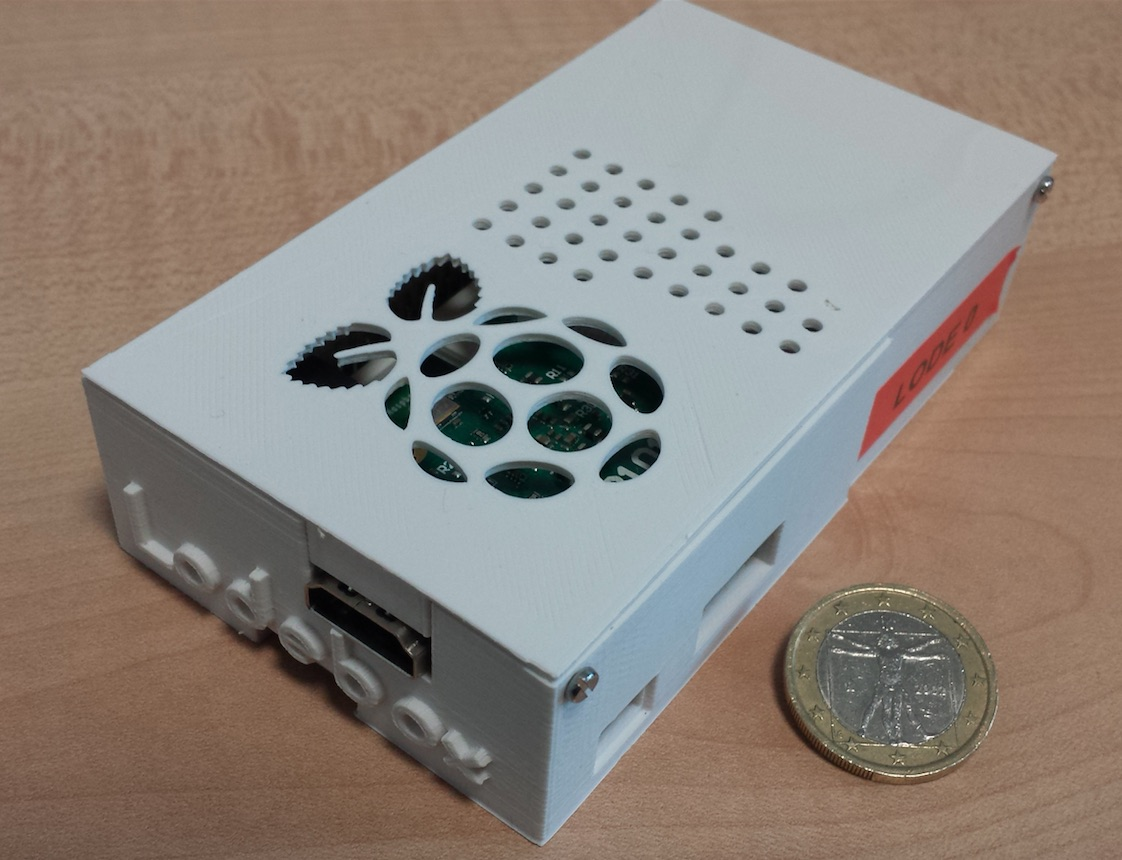
\includegraphics[width=0.3\textwidth]{res/lodebox}
	\caption{\label{fig:lodebox} La scatola di LodeBox.}
\end{wrapfigure}

L'ultima versione di LODE prevede l'utilizzo di una board Raspberry Pi per eseguire il software di acquisizione. Il dispositivo è inserito in una piccola scatola che espone dei connettori verso l'esterno. Tra questi sono presenti un ingresso HDMI per collegare un computer e un'uscita HDMI per collegare un proiettore o uno schermo. Le porte USB permettono di collegare un telecomando e un "dongle" per l'acquisizione dell'audio di un microfono con jack 3,5 mm.

La scatola include un modulo "HDMI to MIPI CSI-2", che permette di convertire il segnale HDMI nel formato seriale della fotocamera. Il video HDMI è infatti acquisito utilizzando la libreria \texttt{PiCamera} per Python, che permette di acquisire il segnale come se si trattasse del video di una fotocamera. La libreria semplifica di molto lo sviluppo, perché espone delle funzioni di alto livello per svolgere operazioni come abilitare l'anteprima del video a schermo intero, la registrazione con un encoder H.264\footnotemark{} con accelerazione hardware e la cattura di screenshot.

\footnotetext{H.264, conosciuto anche come AVC o MPEG-4 Part-10, è il più popolare codec di compressione video. Nato nel 2003, è ancora oggi lo standard de facto in numerosi ambiti, tra cui lo streaming video.}

Sempre in ottica di riduzione dei costi, LodeBox prevede la ripresa del docente tramite una qualsiasi videocamera IP (wireless o cablata) che supporti il protocollo RTSP (Real Time Streaming Protocol). La registrazione avviene sul dispositivo utilizzando \texttt{ffmpeg}/\texttt{avconv}\footnotemark{} in modalità copia (senza ricodifica), richiedendo quindi un uso molto basso di risorse.

\footnotetext{\emph{ffmpeg} è uno strumento estremamente popolare per l'elaborazione di video e audio tramite linea di comando. Supporta numerosi formati, codec e protocolli, e permette di effettuare operazioni quali il muxing, transmuxing, transcoding e altre funzioni più avanzate. \emph{avconv} è un fork di ffmpeg nato per via di divergenze sui metodi di sviluppo, ed è stato incluso per un breve periodo in alcune distribuzioni Linux in sostituzione di ffmpeg.}

Raspberry Pi non prevede spazio di archiviazione interno, e richiede quindi di utilizzare una scheda microSD o una chiavetta USB per memorizzare le registrazioni. Le memorie di tipo flash hanno però vita limitata, a seconda di quanto intensivamente sono utilizzate, e questo riduce di conseguenza l'affidabilità a lungo termine del sistema. Inoltre, la soluzione di usare la porta USB non risulta percorribile, per via delle prestazioni molto scarse che impediscono di registrare tre flussi in contemporanea.

Un altro svantaggio di questa soluzione è il livello di "fault tolerance" in caso di eventi come la disconnessione (volontaria o meno) del cavo HDMI in ingresso. Dato che l'input HDMI è mappato sull'interfaccia della fotocamera, non è previsto che la fotocamera possa essere improvvisamente scollegata. Secondo le prove effettuate, risulta molto difficile rilevare in modo affidabile la disconnessione del cavo HDMI. Nei casi in cui è possibile, non risulta invece fattibile il recupero dell'applicazione, perché le operazioni sulla \texttt{PiCamera} sollevano eccezioni o bloccano indefinitamente l'esecuzione del codice.

Infine, un altro problema è posto dalla presenza del modulo di conversione HDMI-CSI, la cui disponibilità e compatibilità a lungo termine non sono garantite.

\section{Hardware alternativo}
\label{sec:intro_hardware}

Per poter evolvere LodeBox in una soluzione più affidabile e adatta alla produzione e distribuzione, si sono quindi cercate SBC (Single-Board Computer) alternative, preferibilmente pensate per la realizzazione di applicazioni multimediali.

Dal punto di vista tecnico, i principali vincoli per la scelta di una nuova scheda erano la presenza dell'input HDMI e di un encoder H.264 hardware, la possibilità di collegare un microfono e il costo accessibile.

Le soluzioni considerate erano inoltre di tipo pre-industriale, quindi non necessariamente già presenti sul mercato ma personalizzabili per soddisfare i requisiti del prodotto, e offrivano anche determinate garanzie di disponibilità e supporto per un periodo di tempo prolungato.

Molte board con sistema operativo Android soddisfano queste caratteristiche, e consentono in aggiunta di avere a disposizione una piattaforma nota, documentata, di facile sviluppo e per cui sono disponibili molte risorse. In molti casi l'input HDMI è reso disponibile tramite l'interfaccia della fotocamera CSI, da cui deriva la possibilità di acquisire l'input tramite le API di Android per l'accesso alla fotocamera.

